%%%%%%%%%%%%%%%%%%%%%%%%%%%%%%%%%%%%%%%%%%%%%%%%%%%%%%%%%%%%%%%%%%%%%%%
% Sample LaTeX file to get started writing a large document
%%%%%%%%%%%%%%%%%%%%%%%%%%%%%%%%%%%%%%%%%%%%%%%%%%%%%%%%%%%%%%%%%%%%%%%

\documentclass[a4paper,12pt]{book}

%%%%%%%%%%%%%%%%%%%%%%%%%%%%%%%%%%%%%%%%%%%%%%%%%%%%%%%%%%%%%%%%%%%%%%%
% What is the title of the document
%%%%%%%%%%%%%%%%%%%%%%%%%%%%%%%%%%%%%%%%%%%%%%%%%%%%%%%%%%%%%%%%%%%%%%%

\title{A Sample Document}
\date{\today}
\author{Tobias Oetiker\and Peter E. Xample\\
IT Support Gruppe D-ITET (ISG.EE), ETH Z\"urich}

%%%%%%%%%%%%%%%%%%%%%%%%%%%%%%%%%%%%%%%%%%%%%%%%%%%%%%%%%%%%%%%%%%%%%%%
% Load some sensible packages
%%%%%%%%%%%%%%%%%%%%%%%%%%%%%%%%%%%%%%%%%%%%%%%%%%%%%%%%%%%%%%%%%%%%%%%

\usepackage[bookmarks,        % add hyperlinks to the document
            colorlinks,
            plainpages=false]{hyperref}                    
\usepackage[english]{babel}   % use german hyphenation
\usepackage{booktabs}
\usepackage{iftex}              % which tex am I running on
\ifPDFTeX
  \usepackage{lmodern}          % use the Latin Modern Font
  \usepackage[T1]{fontenc}      % understand 8 bit fonts
  \usepackage[latin1]{inputenc} % understand 8 bit latin1 input
\else
   \ifXeTeX
     \usepackage{xltxtra}
   \else 
     \usepackage{luatextra}
   \fi
   \defaultfontfeatures{Ligatures=TeX}
\fi

% \usepackage[utf8]{inputenc} % understand utf8 input
\usepackage{graphicx}         % learn how to include graphics
\usepackage{calc}             % teach latex to calculate
\usepackage{makeidx}          % lets have an index
\makeindex                    % and enable the index
\usepackage{verbatim}         % a better verbatim environment


%%%%%%%%%%%%%%%%%%%%%%%%%%%%%%%%%%%%%%%%%%%%%%%%%%%%%%%%%%%%%%%%%%%%%%%
% define our own page headers
%%%%%%%%%%%%%%%%%%%%%%%%%%%%%%%%%%%%%%%%%%%%%%%%%%%%%%%%%%%%%%%%%%%%%%%

% http://www.ctan.org/tex-archive/macros/latex/contrib/fancyhdr/fancyhdr.pdf

\usepackage{fancyhdr}
\pagestyle{fancy}
\renewcommand{\chaptermark}[1]{\markboth{#1}{}}
\renewcommand{\sectionmark}[1]{\markright{\thesection\ #1}}
\fancyhf{}
\fancyhead[LE,RO]{\bfseries\thepage}
\fancyhead[LO]{\bfseries\rightmark}
\fancyhead[RE]{\bfseries\leftmark}
\fancypagestyle{plain}{%
 \fancyhead{} % get rid of headers
 \renewcommand{\headrulewidth}{0pt} % and the line
}

\addtolength{\headheight}{3pt}

%%%%%%%%%%%%%%%%%%%%%%%%%%%%%%%%%%%%%%%%%%%%%%%%%%%%%%%%%%%%%%%%%%%%%%%
% And so it begins
%%%%%%%%%%%%%%%%%%%%%%%%%%%%%%%%%%%%%%%%%%%%%%%%%%%%%%%%%%%%%%%%%%%%%%%

\begin{document}
\maketitle

\frontmatter % This is all the stuff that comes at the front of the
             % book

\chapter*{Foreword}
Lorem\index{lore} ipsum\index{ipsum} dolor sit amet, consectetuer
adipiscing elit. Etiam eleifend pharetra est. Nunc vulputate nisl quis
leo. In sagittis tristique arcu. Duis varius, enim vel iaculis
sagittis, felis leo ultricies lorem, vitae eleifend velit est quis
nisl. Nulla mattis viverra ipsum. Vestibulum nonummy
adipiscing\index{adipiscing} orci.

\tableofcontents
\listoftables
\listoffigures

\mainmatter

%%%%%%%%%%%%%%%%%%%%%%%%%%%%%%%%%%%%%%%%%%%%%%%%%%%%%%%%%%%%%%%%%%%%%%%
\chapter{And So It Begins}
%%%%%%%%%%%%%%%%%%%%%%%%%%%%%%%%%%%%%%%%%%%%%%%%%%%%%%%%%%%%%%%%%%%%%%%


\section{The Idea}
Duis vitae est. Curabitur congue, tellus vel accumsan interdum, turpis
ligula molestie lacus, a bibendum elit nibh eget lectus. Maecenas ac
dolor. In lacinia lobortis dolor. Morbi et leo. Aliquam erat
volutpat. In nunc elit, scelerisque ac, tincidunt in, mollis id,
velit. Nunc vestibulum. Nullam libero neque, fermentum nec, mollis eu,
rhoncus et, nunc. 

\begin{itemize}
  \item Ene
  \item Mene
  \item Mu
\end{itemize}

Sometimes an enumerated list just makes things so much clearer to the user \ldots
\begin{enumerate}
  \item First
  \item Second
  \item Third
\end{enumerate}

Or if it's more material, maybe a description list is in order.

\begin{description}
  \item[Vivamus] sit amet est dui, vitae tristique metus. Donec felis risus,
  consectetur eu ullamcorper porta, fringilla nec augue.
  \item[Quisqu] gravida
  mauris dui, non iaculis odio. Donec imperdiet ipsum eget nisi rutrum
  varius.
  \item[In adipiscing] enim sit amet justo ultrices nec aliquam orci
  vestibulum. In urna ipsum, pretium in ornare sed, cursus a magna. In hac
  habitasse platea dictumst. Maecenas accumsan,
\end{description}

\begin{table}[htbp]
\begin{center}
\begin{tabular}{|l|l|r|}
\hline
Hello   & World \\ \hline
Test    &
   \begin{minipage}[t]{8cm}
    Vivamus gravida. Nullam consequat luctus libero. Sed interdum, libero
    a eleifend dignissim, justo dolor ultrices erat, in aliquam velit
    massa in magna. Praesent congue diam at neque. Maecenas congue
    purus a.
    \begin{itemize}
      \item Ene
      \item Mene
      \item Mu
    \end{itemize}
    \vspace*{1ex}
   \end{minipage} \\ \hline
\end{tabular}
\end{center}
\caption{A little example table}
\end{table}

\begin{table}[htbp]
\begin{center}
\begin{tabular}{@{}llr@{}} \toprule
\multicolumn{2}{c}{Item} \\ \cmidrule(r){1-2}
Animal & Description & Price (\$)\\ \midrule
Gnat  & per gram  & 13.65 \\
      & each      & 0.01 \\
Gnu   & stuffed   & 92.50 \\
Emu   & stuffed   & 33.33 \\
Armadillo & frozen & 8.99 \\ \bottomrule
\end{tabular}
\end{center}

\begin{center}
\begin{tabular}{@{}llr@{}} \toprule
\multicolumn{2}{c}{Item} \\ \cmidrule(r){1-2}
Animal & Description & Price (\$)\\ \midrule
Gnat  & per gram  & 13.65 \\
      & each      & 0.01 \\
Gnu   & stuffed   & 92.50 \\
Emu   & stuffed   & 33.33 \\
Armadillo & frozen & 8.99 \\ \bottomrule
\end{tabular}
\end{center}
\caption{The effect of booktabs rules on table layout}
\end{table}

Pellentesque luctus bibendum ligula. Suspendisse
consequat imperdiet diam. Duis tincidunt felis a risus. Nullam eu
lacus ac orci convallis nonummy. Pellentesque dictum sollicitudin
purus. Quisque ut ipsum ac orci ultrices ullamcorper. Pellentesque
ornare. Quisque vel tortor. Ut vestibulum, magna in fringilla tempor,
nisl eros rutrum lacus, ut scelerisque magna arcu id mauris. Morbi
semper feugiat sapien.


\section{The Implementation}


Vivamus gravida. Nullam consequat luctus libero. Sed interdum, libero
massa in magna. Praesent congue diam at neque. Maecenas congue purus a
nunc. Donec placerat purus ut nisi. Vestibulum fermentum hendrerit
turpis. Cum sociis natoque penatibus et magnis dis parturient montes,
nascetur ridiculus mus. Sed et orci ut sapien porta
scelerisque. Aenean placerat nunc vel mi. 

\begin{figure}[hbtp]
\begin{center}
\framebox{\Huge\textbf{Big!}}
\end{center}
\caption{A big Text}
\end{figure}

Vivamus ultrices ipsum ut
kdsfhk kjdhf khweiu fsdfhlkhs
nibh. Nam laoreet nonummy dui. Suspendisse in augue. 

\section{The Graphic}

blala lsldk dkldshjfo oewii fjoehw osdofojhoef ncowihjeohow oico w. iwfoiefh
nkskfjhoewi blalal graphic \ref{fig:gauss} on \pageref{fig:gauss}, blaal
blal blkaks.

\begin{figure}[hbtp]
\begin{center}
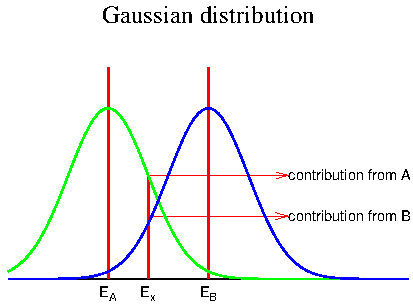
\includegraphics[width=0.8\textwidth]{gauss}
\end{center}
\caption{The Gauss plott}
\label{fig:gauss}
\end{figure}
%%%%%%%%%%%%%%%%%%%%%%%%%%%%%%%%%%%%%%%%%%%%%%%%%%%%%%%%%%%%%%%%%%%%%%%
% The Appendix
%%%%%%%%%%%%%%%%%%%%%%%%%%%%%%%%%%%%%%%%%%%%%%%%%%%%%%%%%%%%%%%%%%%%%%%

\appendix

\chapter{Don't Forget this}

Sed feugiat, eros ut gravida lacinia, massa arcu ornare dolor, id
molestie eros diam ac magna. Fusce viverra erat pharetra quam. Morbi
aliquet aliquam magna. Sed eleifend nunc id dolor. Proin ligula felis,
consequat vel, convallis non, consequat sed, neque. Quisque euismod,
mi in iaculis convallis, velit mauris auctor leo, sed nonummy sapien
sapien non arcu. Pellentesque sagittis laoreet nunc.

\chapter{The Source}

{\tiny \verbatiminput{sample.tex}}

%%%%%%%%%%%%%%%%%%%%%%%%%%%%%%%%%%%%%%%%%%%%%%%%%%%%%%%%%%%%%%%%%%%%%%%
% Bibliography
%%%%%%%%%%%%%%%%%%%%%%%%%%%%%%%%%%%%%%%%%%%%%%%%%%%%%%%%%%%%%%%%%%%%%%%

\begin{thebibliography}{99}
\addcontentsline{toc}{chapter}{\bibname} 
\bibitem{manual} Leslie Lamport.  \newblock \emph{{\LaTeX:} A Document
    Preparation System}.  \newblock Addison-Wesley, Reading,
  Massachusetts, second edition, 1994, ISBN~0-201-52983-1.
  
\bibitem{texbook} Donald~E. Knuth.  \newblock \textit{The \TeX{}book,}
  Volume~A of \textit{Computers and Typesetting}, Addison-Wesley,
  Reading, Massachusetts, second edition, 1984, ISBN~0-201-13448-9.

\bibitem{companion} Frank Mittelbach, Michel Goossens, Johannes Braams,
  David Carlisle, Chris Rowley.  \newblock \emph{The {\LaTeX} Companion, (2nd
  Edition)}.  \newblock Addison-Wesley, Reading, Massachusetts, 2004,
  ISBN~0-201-36299-6.

\bibitem{graphicscompanion} Michel Goossens, Sebastian Rahtz and Frank
  Mittelbach.  \newblock \emph{The {\LaTeX} Graphics Companion}.  \newblock
  Addison-Wesley, Reading, Massachusetts, 1997, ISBN~0-201-85469-4.
 
\end{thebibliography}

%%%%%%%%%%%%%%%%%%%%%%%%%%%%%%%%%%%%%%%%%%%%%%%%%%%%%%%%%%%%%%%%%%%%%%
% The Index
%%%%%%%%%%%%%%%%%%%%%%%%%%%%%%%%%%%%%%%%%%%%%%%%%%%%%%%%%%%%%%%%%%%%%%
% after compiling two times, run 'makeindex sample' to generate
% the index file
\printindex

%%%%%%%%%%%%%%%%%%%%%%%%%%%%%%%%%%%%%%%%%%%%%%%%%%%%%%%%%%%%%%%%%%%%%%
% Stuff that goes into the back of the book
%%%%%%%%%%%%%%%%%%%%%%%%%%%%%%%%%%%%%%%%%%%%%%%%%%%%%%%%%%%%%%%%%%%%%%
\backmatter

\chapter{Production Notes}

Etiam fermentum velit nec ligula. Fusce dapibus lacus quis nibh. Duis
consequat metus non dolor. Fusce a odio feugiat turpis sagittis
pulvinar. Sed ac dui. Nulla quis augue convallis orci tristique
vestibulum. Phasellus molestie. Etiam quis risus. Maecenas
volutpat. Praesent nec dolor sed mauris vulputate gravida. Aliquam
ullamcorper diam eget mi. Donec accumsan tincidunt ligula. Praesent
sodales tortor eget ligula. Etiam dolor elit, placerat id, rhoncus
eget, tincidunt sit amet, dui. dkdkal weidke keeidiu ekeek, dkelkwj, 
kdkdkele, ekeekkdkdk dkekekldl, ekkeiidid, ekekwood, ekekeidi
kekelsfoi, lwefijwfjl, ifwiikddk, kdsfljfl elwjfoieo ioiwruo4fc
k4ejfouja fjowieu odiidkdlsjljfoi kjsdlfjwoijc

\end{document}


Local Variables:
% ispell-local-dictionary: "deutsch8"
mode: flyspell
End:
